\documentclass[a4paper, 14pt]{extarticle}
\usepackage[english,russian]{babel}
\usepackage[T1]{fontenc}
\usepackage[utf8]{inputenc}
\usepackage{fontspec}
\usepackage{indentfirst}
\usepackage{enumitem}
\usepackage{graphicx}
\usepackage[
  left=20mm,
  right=10mm,
  top=20mm,
  bottom=20mm
]{geometry}
\usepackage{parskip}
\usepackage{titlesec}
\usepackage{xurl}
\usepackage{hyperref}
\usepackage{float}
\usepackage[
  figurename=Рисунок,
  labelsep=endash,
  justification=centering
]{caption}
\usepackage[outputdir=build, newfloat]{minted}
\usepackage{chngcntr}

\selectlanguage{russian}

\hypersetup{
  colorlinks=true,
  linkcolor=black,
  filecolor=blue,
  urlcolor=blue,
}

\renewcommand*{\labelitemi}{---}
\setmainfont{Times New Roman}
\setmonofont{JetBrains Mono}[
  SizeFeatures={Size=11},
]

\newenvironment{code}{\captionsetup{type=figure}}{}
\BeforeBeginEnvironment{code}{\bigskip}
\AfterEndEnvironment{code}{\bigskip}

\setminted{
  fontsize=\footnotesize,
}

\setlength{\parskip}{6pt}

\setlength{\parindent}{1.25cm}
\setlist[itemize]{itemsep=0em,topsep=0em,parsep=0em,partopsep=0em,leftmargin=2.0cm,wide}
\setlist[enumerate]{itemsep=0em,topsep=0em,parsep=0em,partopsep=0em,leftmargin=2.0cm,wide}

\renewcommand{\thesection}{\indent\arabic{section}.}
\renewcommand{\thesubsection}{\indent\thesection\arabic{subsection}.}
\renewcommand{\thesubsubsection}{\indent\thesubsection\arabic{subsubsection}.}

\titleformat{\section}{\normalfont\bfseries}{\thesection}{0.5em}{}
\titleformat{\subsection}{\normalfont\bfseries}{\thesubsection}{0.5em}{}
\titleformat{\subsubsection}{\normalfont\bfseries}{\thesubsubsection}{0.5em}{}

\titleformat*{\section}{\normalfont\bfseries}
\titleformat*{\subsection}{\normalfont\bfseries}
\titleformat*{\subsubsection}{\normalfont\bfseries}

\titlespacing{\section}{\parindent}{\parskip}{\parskip}
\titlespacing{\subsection}{\parindent}{\parskip}{\parskip}
\titlespacing{\subsubsection}{\parindent}{\parskip}{\parskip}

\begin{document}

\begin{titlepage}
  \vspace{0pt plus2fill}
  \noindent

  \vspace{0pt plus6fill}
  \begin{center}
    {
    \bfseries
    Министерство науки и высшего образования Российской Федерации
    {
    \scriptsize
    ФЕДЕРАЛЬНОЕ ГОСУДАРСТВЕННОЕ АВТОНОМНОЕ ОБРАЗОВАТЕЛЬНОЕ УЧРЕЖДЕНИЕ ВЫСШЕГО
    ОБРАЗОВАНИЯ
    }
    «Национальный исследовательский университет ИТМО»

    (Университет ИТМО)

    \begin{minipage}[t]{0.42\textwidth}
      \vspace*{0pt}
      \begin{flushright}
        Факультет

        Образовательная программа
      \end{flushright}
    \end{minipage}
    \begin{minipage}[t]{0.57\textwidth}
      \vspace*{0pt}
      \begin{flushright}
        Инфокоммуникационных технологий

        11.03.02 Программирование в инфокоммуникационных системах
      \end{flushright}
    \end{minipage}
    }

    \vspace{0pt plus5fill}

    \LARGE{
      ОТЧЕТ

      по лабораторной работе 3

      по дисциплине \textbf{<<Разработка баз данных>>}
    }
  \end{center}

  \vspace{0pt plus4fill}
  \begin{flushright}
    Выполнил: \textbf{студент группы K33211 Швалов Д. А.}

    Проверил: \textbf{ст. преподаватель Осетрова И.С.}
  \end{flushright}

  \vspace{0pt plus8fill}
  \begin{center}
    Санкт-Петербург

    2024
  \end{center}
\end{titlepage}

\setcounter{page}{2}

\linespread{1.5}
\renewcommand{\baselinestretch}{1.5}

\section*{\large{Лабораторная работа №3 <<Создание индексов и диаграмм>>}}

\section{Цель работы}

Создание индексов и диаграмм.

\section{Задачи, решаемые при выполнении работы}

\begin{enumerate}[leftmargin=*]
  \item Создание индекса с помощью конструктора таблиц.
  \item Создание индекса в Query Editor: шаблоны.
  \item Создание индекса в Query Editor: код T-SQL.
  \item Изменение индекса.
  \item Удаление индекса.
  \item Построение диаграмм базы данных.
  \item Создание составного индекса.
\end{enumerate}

\section{Объект исследования}

Создание индексов и диаграмм в СУБД \foreignlanguage{english}{Microsoft SQL
Server} с помощью \foreignlanguage{english}{Microsoft SQL Server Management
Studio (SSMS)}.

\section{Исходные данные}

\begin{itemize}
  \item методические указания к лабораторной работе;
  \item СУБД Microsoft SQL Server;
  \item Microsoft SQL Server Management Studio;
  \item база данных ApressFinancial.
\end{itemize}

\section{Выполнение работы}

\subsection{Первая задача}

\subsubsection{Открытие настроек индексов}

Помощью контекстного меню (рисунок \ref{fig:task-1-1}) был открыт конструктор
таблиц. После этого с помощью кнопки <<\foreignlanguage{english}{Manage Indexes
and Keys}>> на панели инструментов (рисунок \ref{fig:task-1-2}) были открыты
настройки индексов, показанные на рисунке \ref{fig:task-1-3}.

\begin{figure}[H]
  \centering
  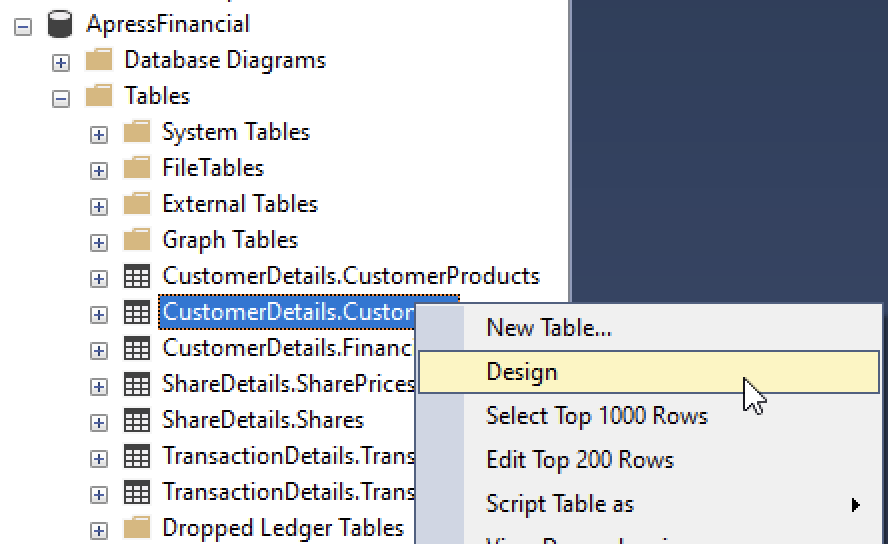
\includegraphics[width=0.6\textwidth]{images/task-1/1.png}
  \caption{Открытие дизайнера таблиц с помощью контекстного меню}
  \label{fig:task-1-1}
\end{figure}

\begin{figure}[H]
  \centering
  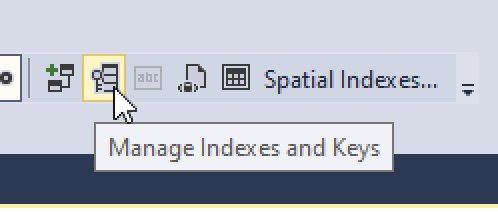
\includegraphics[width=0.4\textwidth]{images/task-1/2.png}
  \caption{Открытие настроек индексов}
  \label{fig:task-1-2}
\end{figure}

\begin{figure}[H]
  \centering
  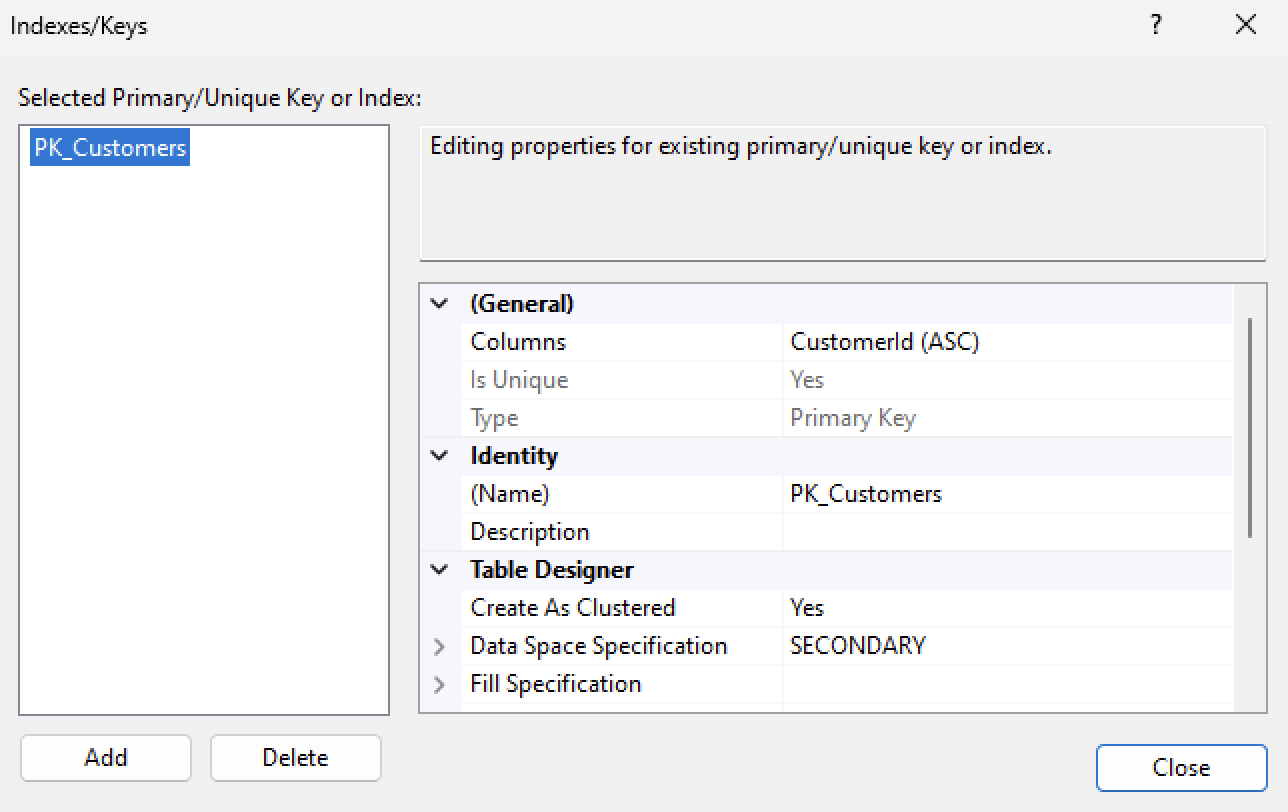
\includegraphics[width=0.8\textwidth]{images/task-1/3.png}
  \caption{Окно настроек индексов}
  \label{fig:task-1-3}
\end{figure}

\subsubsection{Создание индекса}

С помощью кнопки <<Add>> был создан новый индекс. Для него было указано имя
<<\foreignlanguage{english}{IX\_Customers\_CustomerId}>>, установлен порядок
сортировки по возрастанию, установлена опция <<\foreignlanguage{english}{Is
Unique}>> (рисунок \ref{fig:task-1-4}). После этого в SSMS для таблицы
<<\foreignlanguage{english}{Customers}>> появился новый индекс.

\begin{figure}[H]
  \centering
  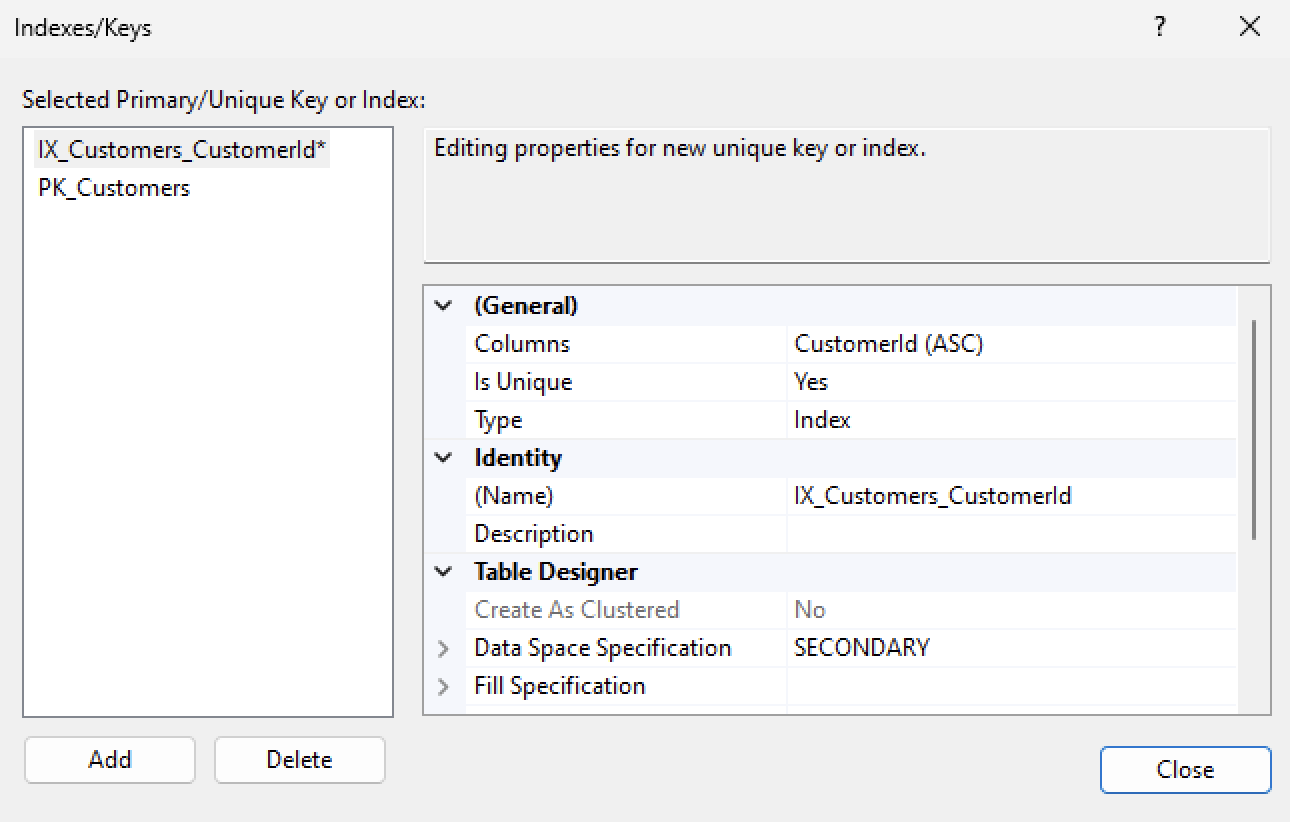
\includegraphics[width=0.8\textwidth]{images/task-1/4.png}
  \caption{Создание индекса для таблицы <<Customers>>}
  \label{fig:task-1-4}
\end{figure}

\subsection{Вторая задача}

\subsubsection{Создание индекса с помощью шаблона}

С помощью кнопки <<\foreignlanguage{english}{Template Explorer}>> на панели
инструментов (рисунок \ref{fig:task-2-1}) был открыт обозреватель шаблонов. В
нем в узле <<\foreignlanguage{english}{Index}>> был выбран шаблон с именем
<<\foreignlanguage{english}{Create Index Basic}>> (рисунок \ref{fig:task-2-2}).
После этого в редакторе запросов был сгенерирован запрос, показанный на рисунке
\ref{fig:task-2-3}.

\begin{figure}[H]
  \centering
  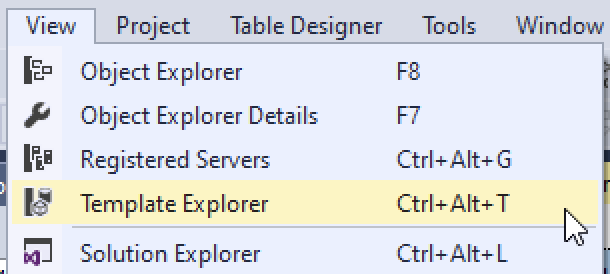
\includegraphics[width=0.4\textwidth]{images/task-2/1.png}
  \caption{Кнопка открытия обозревателя шаблонов}
  \label{fig:task-2-1}
\end{figure}

\begin{figure}[H]
  \centering
  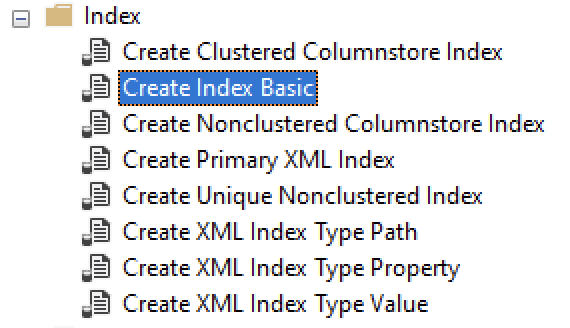
\includegraphics[width=0.5\textwidth]{images/task-2/2.png}
  \caption{Шаблон для создания индекса}
  \label{fig:task-2-2}
\end{figure}

\begin{figure}[H]
  \centering
  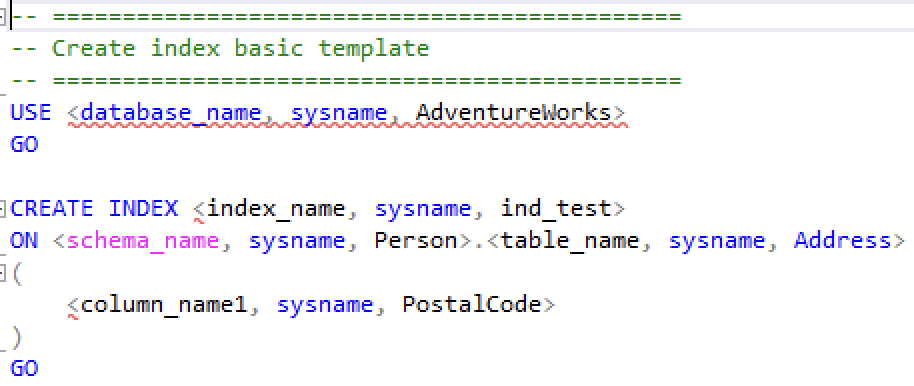
\includegraphics[width=\textwidth]{images/task-2/3.png}
  \caption{Сгенерированный запрос}
  \label{fig:task-2-3}
\end{figure}

\subsubsection{Настройка переменных шаблона}

Согласно заданию, для шаблона были настроены переменные так, как это показано на
рисунке \ref{fig:task-2-4}. После сохранения измененных переменных запрос принял
вид, показанный на рисунке \ref{fig:task-2-5}. После выполнения сгенерированного
запроса в обозревателе появился новый индекс.

\begin{figure}[H]
  \centering
  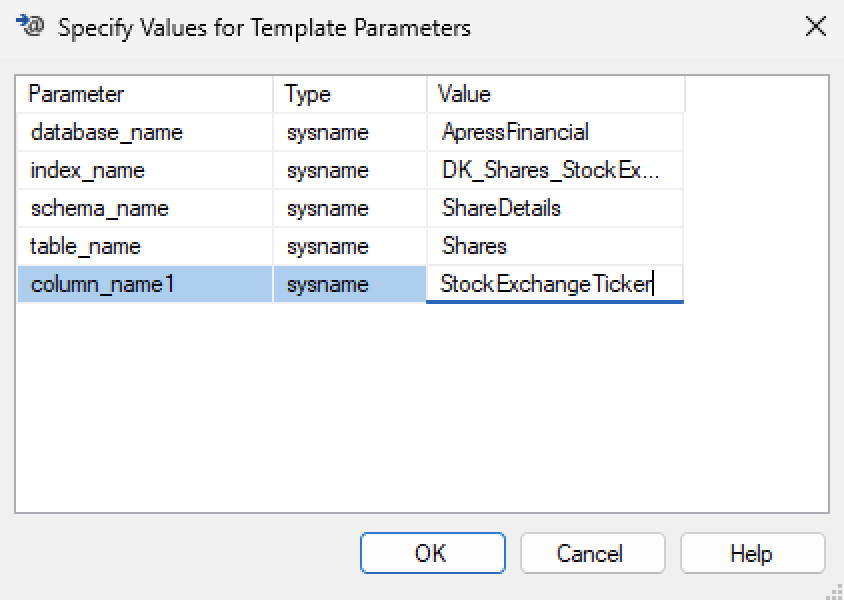
\includegraphics[width=0.7\textwidth]{images/task-2/4.png}
  \caption{Окно настройки переменных шаблона}
  \label{fig:task-2-4}
\end{figure}

\begin{figure}[H]
  \centering
  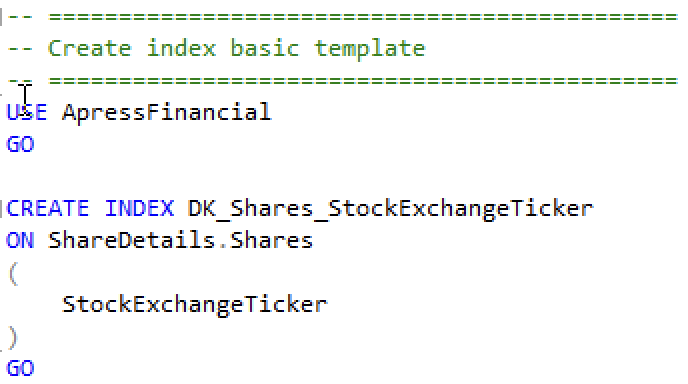
\includegraphics[width=0.7\textwidth]{images/task-2/5.png}
  \caption{Сгенерированный запрос}
  \label{fig:task-2-5}
\end{figure}

\subsubsection{Просмотр свойств индекса}

С помощью контекстного меню, как показано на рисунке \ref{fig:task-2-6}, были
открыты свойства индекса. На рисунке \ref{fig:task-2-7} показана страница
<<\foreignlanguage{english}{Fragmentation}>>, представляющая наибольший интерес.
Поскольку данных в таблице нет, то и фрагментации данных не наблюдается.

\begin{figure}[H]
  \centering
  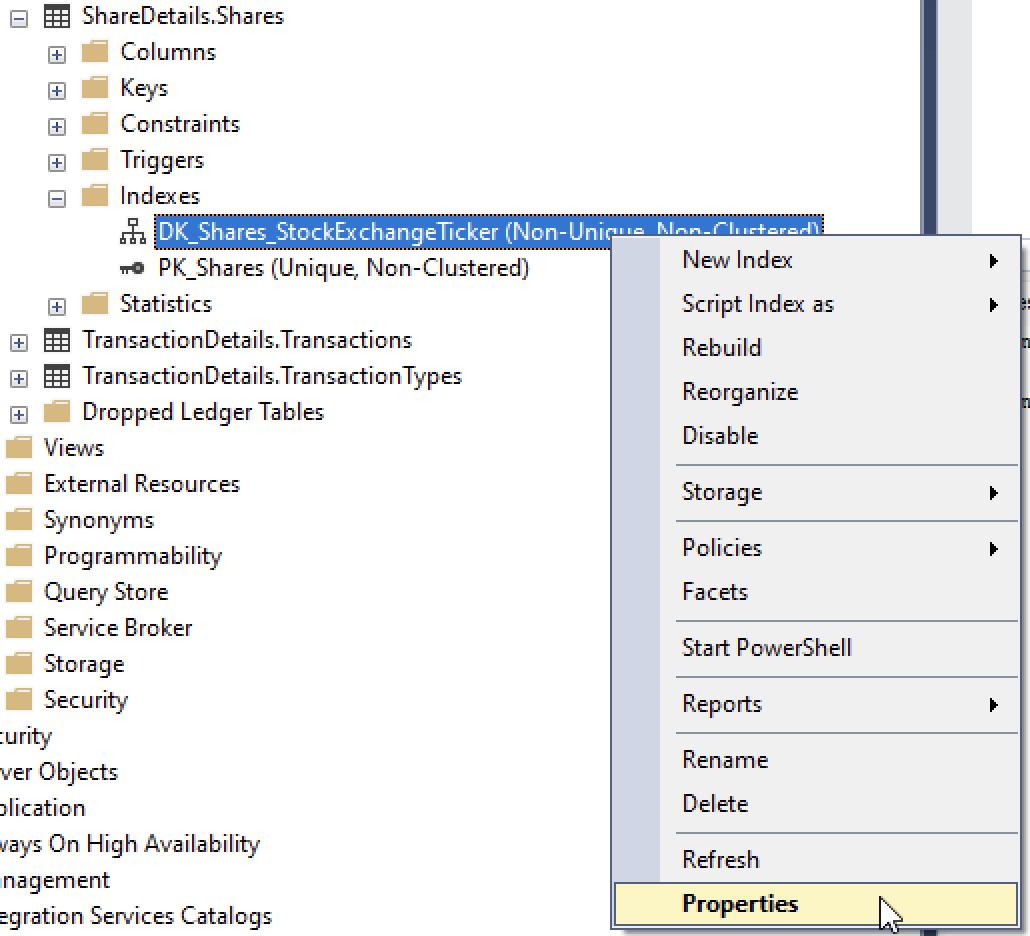
\includegraphics[width=0.7\textwidth]{images/task-2/6.png}
  \caption{Кнопка открытия свойств индекса}
  \label{fig:task-2-6}
\end{figure}

\begin{figure}[H]
  \centering
  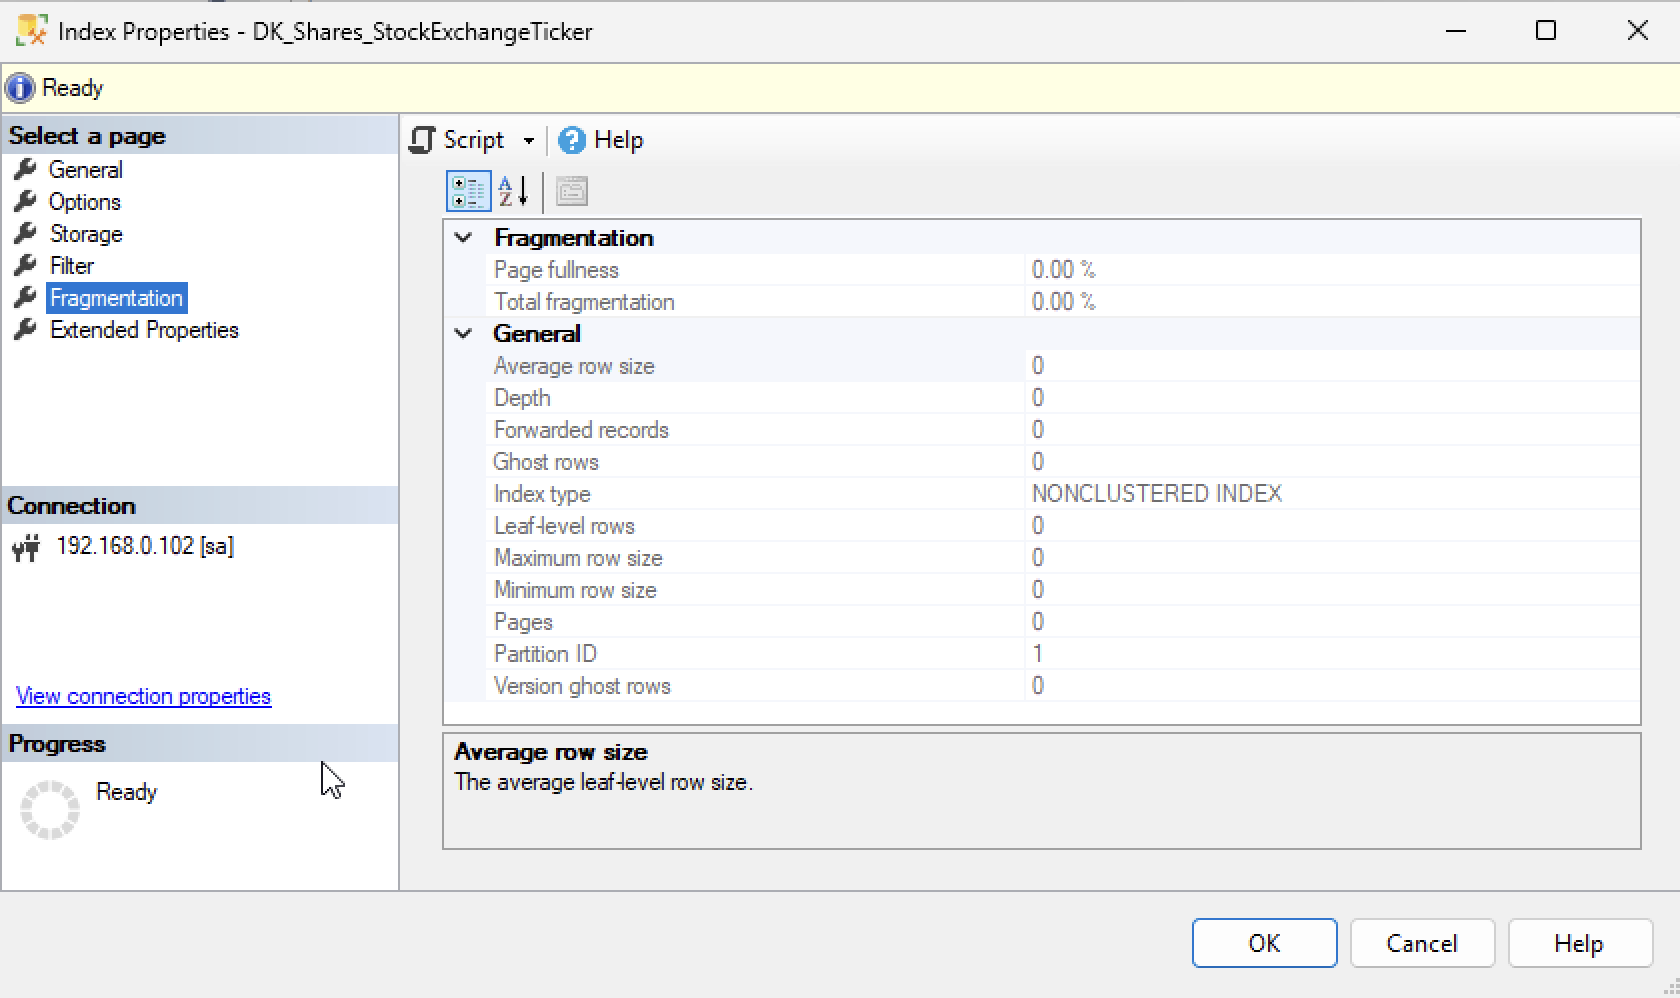
\includegraphics[width=\textwidth]{images/task-2/7.png}
  \caption{Свойства индекса}
  \label{fig:task-2-7}
\end{figure}

\subsection{Третья задача}

\subsubsection{Создание кластеризованного индекса}

На рисунке \ref{fig:task-3-1} показан запрос для создания уникального
кластеризованного индекса <<\foreignlanguage{english}{IX\_TransactionTypes}>>
для таблицы <<\foreignlanguage{english}{TransactionTypes}>> по столбцу
<<\foreignlanguage{english}{TransactionTypeId}>>. После выполнения данного
запроса, как показано на рисунке \ref{fig:task-3-2}, индекс появился в
интерфейсе SSMS.

\begin{figure}[H]
  \centering
  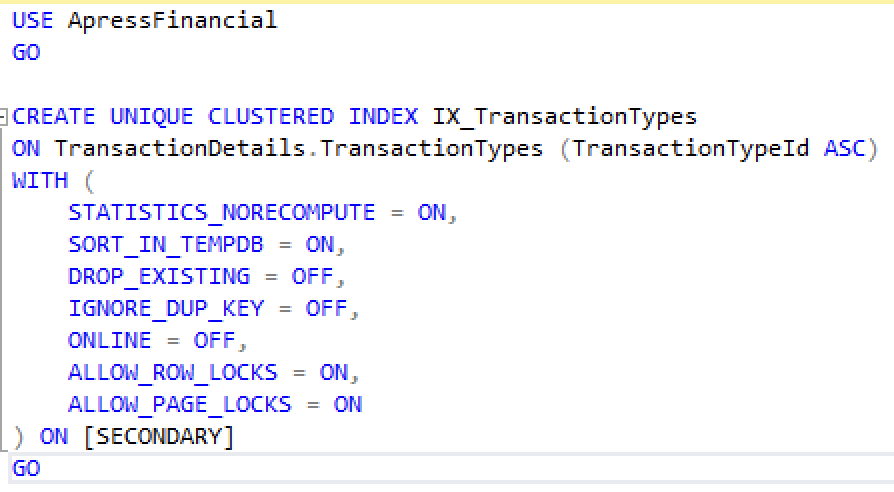
\includegraphics[width=\textwidth]{images/task-3/1.png}
  \caption{Запрос для создания индекса в таблице <<TransactionTypes>>}
  \label{fig:task-3-1}
\end{figure}

\begin{figure}[H]
  \centering
  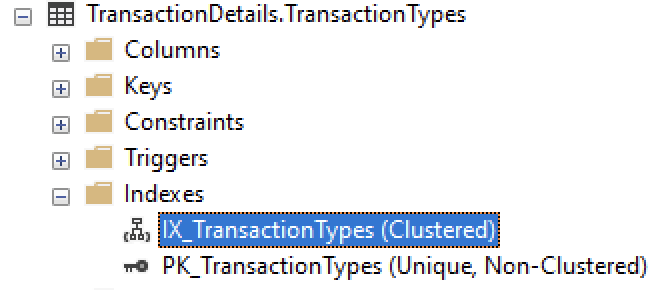
\includegraphics[width=0.6\textwidth]{images/task-3/2.png}
  \caption{Созданный индекс}
  \label{fig:task-3-2}
\end{figure}

\subsubsection{Создание кластеризованного индекса}

На рисунке \ref{fig:task-3-3} показан запрос для создания неуникального
некластеризованного индекса
<<\foreignlanguage{english}{IX\_Transactions\_TType}>> для таблицы
<<\foreignlanguage{english}{Transactions}>> по столбцу
<<\foreignlanguage{english}{TransactionTypeId}>>. После выполнения данного
запроса, как показано на рисунке \ref{fig:task-3-4}, индекс появился в
интерфейсе SSMS.

\begin{figure}[H]
  \centering
  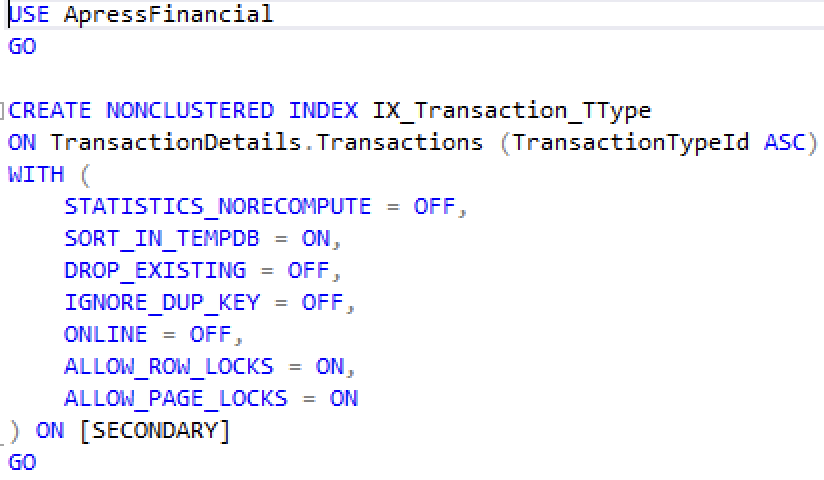
\includegraphics[width=\textwidth]{images/task-3/3.png}
  \caption{Запрос для создания индекса в таблице <<Transactions>>}
  \label{fig:task-3-3}
\end{figure}

\begin{figure}[H]
  \centering
  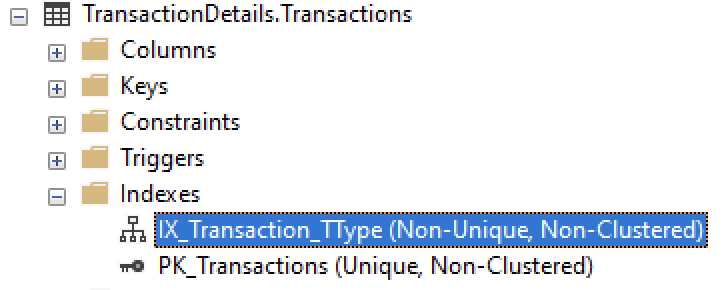
\includegraphics[width=0.6\textwidth]{images/task-3/4.png}
  \caption{Созданный индекс}
  \label{fig:task-3-4}
\end{figure}

\subsection{Четвертая задача}

\subsubsection{Создание индекса}

На рисунке \ref{fig:task-4-1} показан запрос для создания индекса
<<\foreignlanguage{english}{IX\_CustTransDate}>> в таблице
<<\foreignlanguage{english}{Transactions}>> по столбцам
<<\foreignlanguage{english}{CustomerId}>> и
<<\foreignlanguage{english}{DateEntered}>>. После выполнения данного запроса,
как показано на рисунке \ref{fig:task-4-2}, индекс появился в SSMS.

\begin{figure}[H]
  \centering
  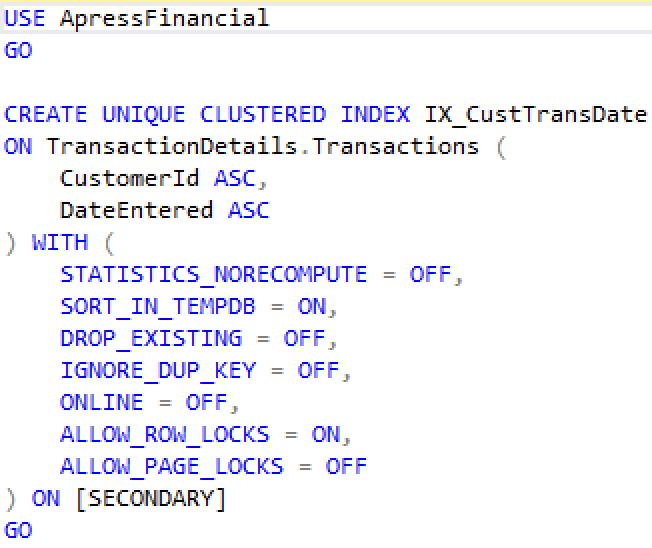
\includegraphics[width=0.7\textwidth]{images/task-4/1.png}
  \caption{Запрос для создания индекс}
  \label{fig:task-4-1}
\end{figure}

\begin{figure}[H]
  \centering
  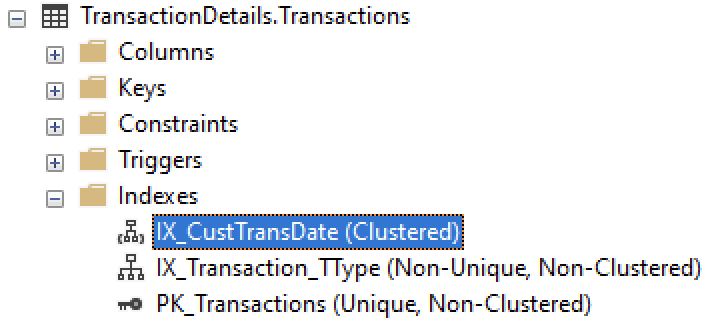
\includegraphics[width=0.6\textwidth]{images/task-4/2.png}
  \caption{Созданный индекс}
  \label{fig:task-4-2}
\end{figure}

\subsubsection{Изменение индекса}

С помощью запроса, показанного на рисунке \ref{fig:task-4-3}, индекс
<<\foreignlanguage{english}{IX\_CustTransDate}>> был изменен: для столбца
<<\foreignlanguage{english}{DateEntered}>> порядок был изменен с
<<\foreignlanguage{english}{ASC}>> на <<\foreignlanguage{english}{DESC}>>.
Также для того, чтобы индекс был обновлен, был установлен параметр
<<\foreignlanguage{english}{DROP\_EXISTING}>> в значение
<<\foreignlanguage{english}{ON}>>. После этого, как видно на рисунке
\ref{fig:task-4-4}, порядок столбца был изменен.

\begin{figure}[H]
  \centering
  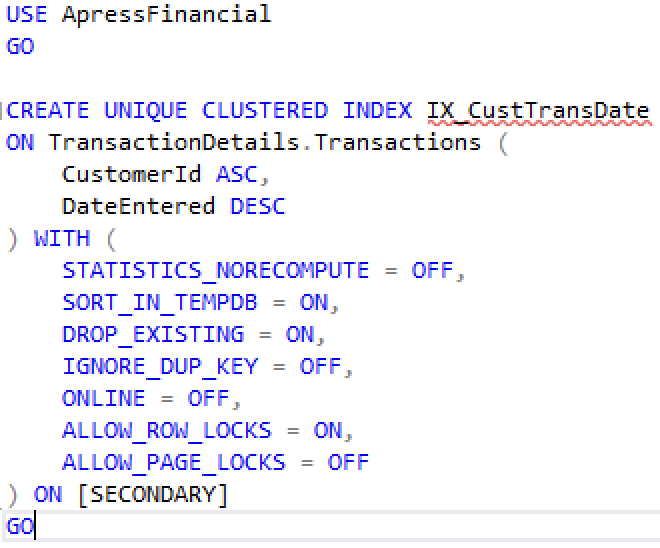
\includegraphics[width=0.7\textwidth]{images/task-4/3.png}
  \caption{Запрос для изменения индекса}
  \label{fig:task-4-3}
\end{figure}

\begin{figure}[H]
  \centering
  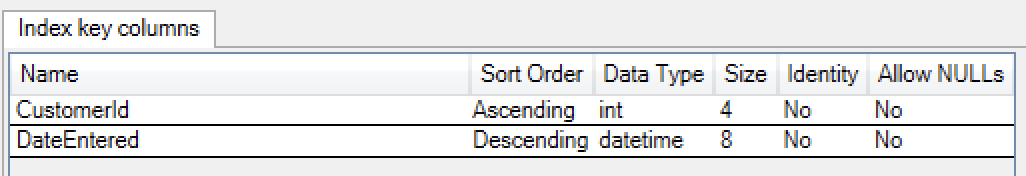
\includegraphics[width=\textwidth]{images/task-4/4.png}
  \caption{Порядок столбцов индекса}
  \label{fig:task-4-4}
\end{figure}

\subsection{Пятая задача}

\subsubsection{Удаление индекса}

На рисунке \ref{fig:task-5-1} представлен запрос для удаления индекса
<<\foreignlanguage{english}{IX\_CustTransDate}>> из таблицы
<<\foreignlanguage{english}{Transactions}>>. Как видно на рисунке
\ref{fig:task-5-2}, после выполнения данного запроса индекс был удален.

\begin{figure}[H]
  \centering
  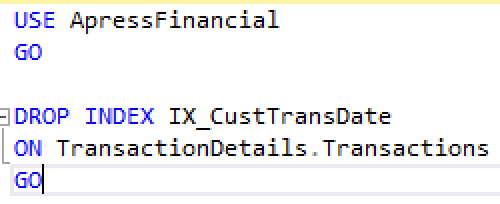
\includegraphics[width=0.6\textwidth]{images/task-5/1.png}
  \caption{Запрос для удаления индекса}
  \label{fig:task-5-1}
\end{figure}

\begin{figure}[H]
  \centering
  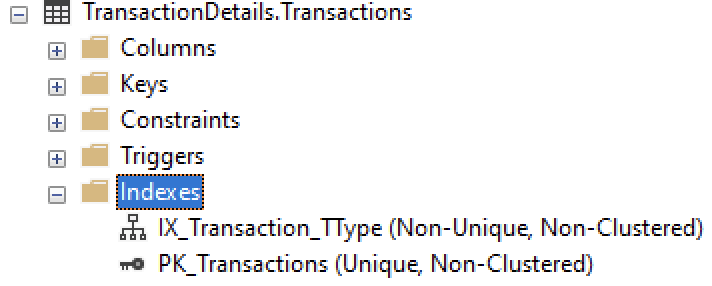
\includegraphics[width=0.6\textwidth]{images/task-5/2.png}
  \caption{Результат выполнения запроса}
  \label{fig:task-5-2}
\end{figure}

\subsection{Шестая задача}

\subsubsection{Включение поддержки диаграммы}

Для базы данных <<\foreignlanguage{english}{ApressFinancial}>> с помощью узла
<<\foreignlanguage{english}{Database Diagrams}>> (рисунок \ref{fig:task-6-1}), а
также с помощью диалогового окна (рисунок \ref{fig:task-6-2}) была включена
поддержка диаграмм.

\begin{figure}[H]
  \centering
  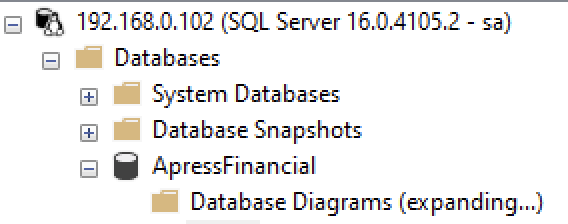
\includegraphics[width=0.6\textwidth]{images/task-6/1.png}
  \caption{Узел <<Database Diagrams>>}
  \label{fig:task-6-1}
\end{figure}

\begin{figure}[H]
  \centering
  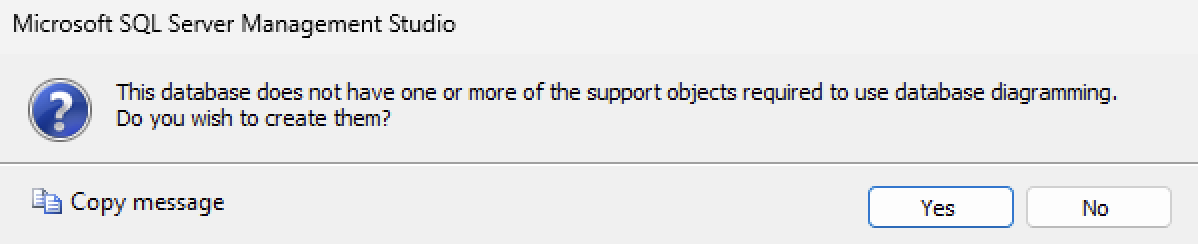
\includegraphics[width=\textwidth]{images/task-6/2.png}
  \caption{Диалоговое окно создания диаграммы}
  \label{fig:task-6-2}
\end{figure}

\subsubsection{Создание диаграммы}

С помощью контекстного меню, показанного на рисунке \ref{fig:task-6-3}, было
открыто окно для добавления таблиц в диаграмму (рисунок \ref{fig:task-6-4}).
После этого на экране появилась диаграмма, показанная на рисунке
\ref{fig:task-6-5}. От диаграммы, представленной в предыдущей лабораторной
работе, она отличается следующим. У созданной диаграммы из всех связей
присутствуют только связи между таблицами
<<\foreignlanguage{english}{Transactions}>> и
<<\foreignlanguage{english}{Customers}>>,
<<\foreignlanguage{english}{Transactions}>> и
<<\foreignlanguage{english}{Shares}>>. Все остальные связи отсутствуют. Сами
таблицы являются идентичными.

\begin{figure}[H]
  \centering
  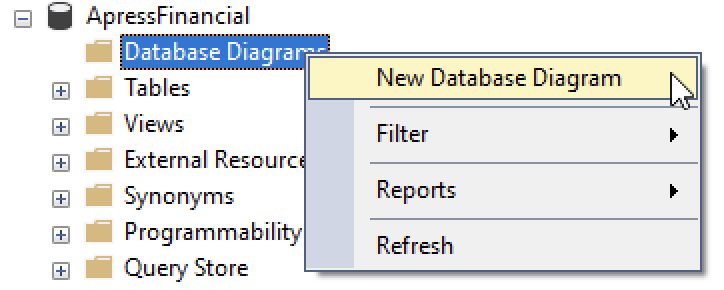
\includegraphics[width=0.5\textwidth]{images/task-6/3.png}
  \caption{Меню создания диаграммы}
  \label{fig:task-6-3}
\end{figure}

\begin{figure}[H]
  \centering
  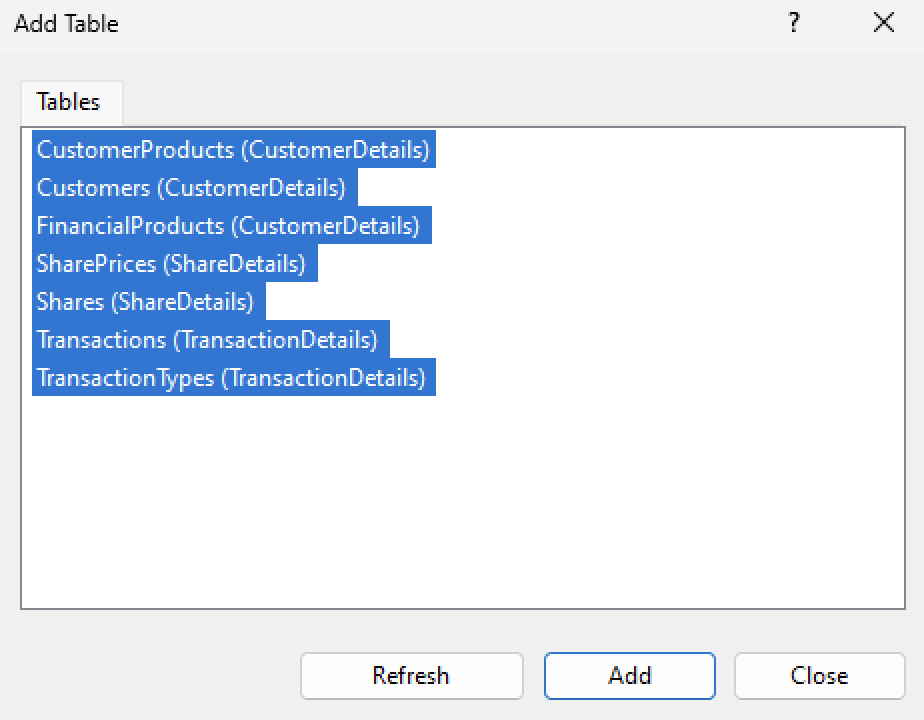
\includegraphics[width=0.5\textwidth]{images/task-6/4.png}
  \caption{Добавление таблиц в диаграмму}
  \label{fig:task-6-4}
\end{figure}

\begin{figure}[H]
  \centering
  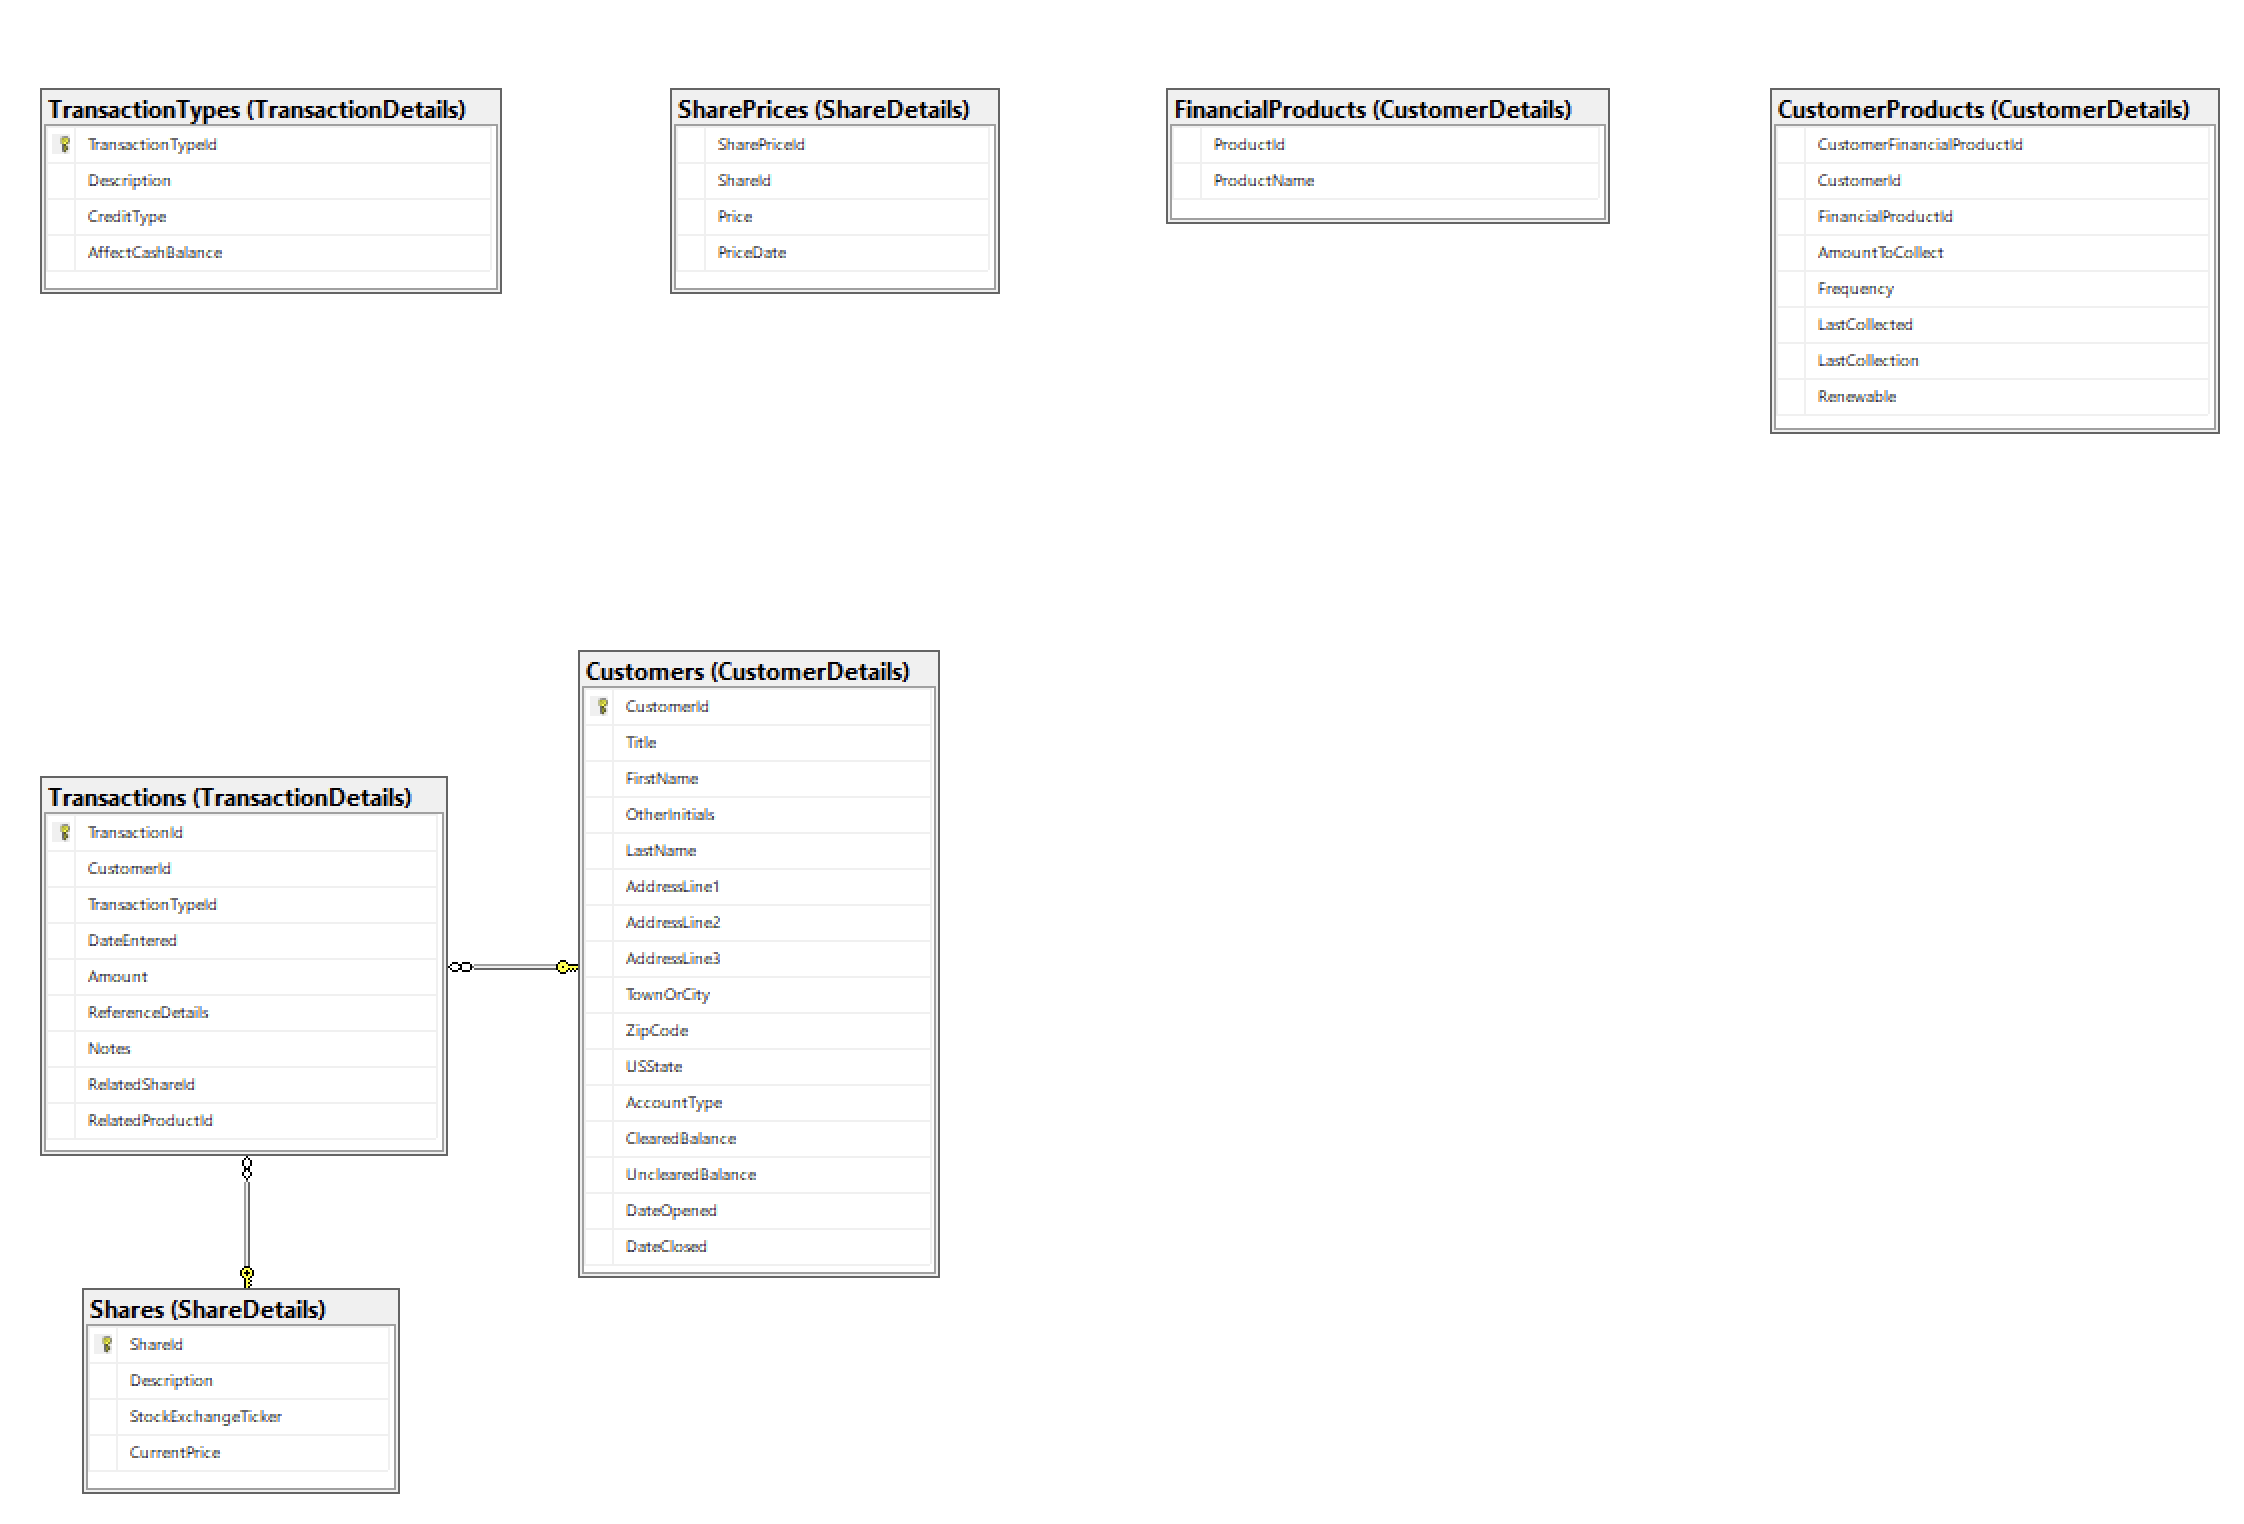
\includegraphics[width=\textwidth]{images/task-6/5.png}
  \caption{Созданная диаграмма}
  \label{fig:task-6-5}
\end{figure}

\subsection{Седьмая задача}

\subsubsection{Создание составного индекса}

С помощью запроса, представленного на рисунке \ref{fig:task-7-1}, был создан
индекс <<\foreignlanguage{english}{IX\_Customers\_LastNameZip}>> для таблицы
<<\foreignlanguage{english}{Customers}>>. В качестве индексируемых столбцов были
выбраны столбцы <<\foreignlanguage{english}{LastName}>> и
<<\foreignlanguage{english}{ZipCode}>>, для которых была установлена сортировка
по возрастанию. Индекс был создан неуникальным, поскольку пара фамилия и
почтовый индекс не обязательна быть уникальной (например, для родственников).
Также индекс был создан как некластеризованный, поскольку данные столбцы не
являются идентификаторами. После выполнения данного запроса в интерфейсе SSMS
появился созданный индекс (рисунок \ref{fig:task-7-2}).

\begin{figure}[H]
  \centering
  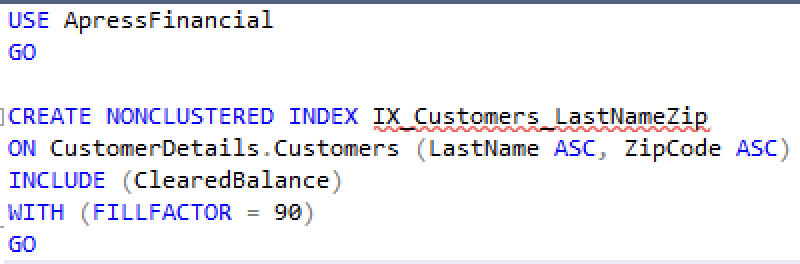
\includegraphics[width=0.8\textwidth]{images/task-7/1.png}
  \caption{Запрос для создания индекса}
  \label{fig:task-7-1}
\end{figure}

\begin{figure}[H]
  \centering
  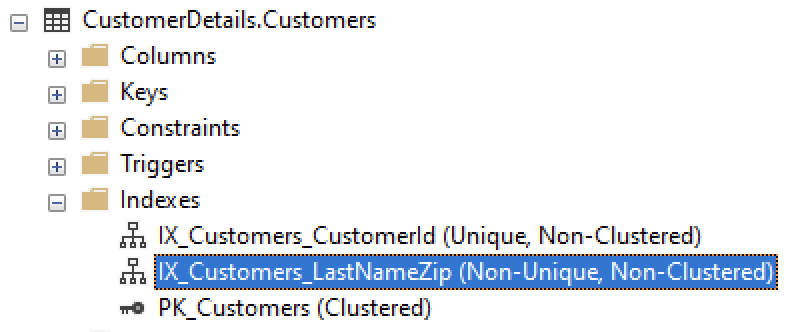
\includegraphics[width=0.7\textwidth]{images/task-7/2.png}
  \caption{Созданный индекс}
  \label{fig:task-7-2}
\end{figure}

\section{Выводы и анализ результатов работы}

В данной лабораторной работе изучены способы создания индексов с помощью
конструктора таблиц SSMS и с помощью запросов на языке T-SQL, а также способ
создания диаграмм.

Цель, поставленная в начале работы, достигнута, задачи выполнены.

\end{document}
